\documentclass[a4paper]{article}
%\usepackage[T2A]{fontenc}
\usepackage[utf8]{inputenc} %% ваша любимая кодировка здесь
\usepackage{mathtext}
\usepackage[english,russian]{babel} %% это необходимо для включения переносов
\usepackage{float}
\usepackage{graphicx}
\usepackage[14pt]{extsizes}
%\usepackage{times}
%\usepackage{cyrtimes}
\usepackage{vmargin}
%\setmarginsrb{0.5cm}{0.5cm}{0.5cm}{0.5cm}{0pt}{0mm}{0pt}{13mm}
\usepackage{indentfirst}
\usepackage{amsmath}
\usepackage{cmap}          % русский поиск в pdf
\usepackage{amsfonts}
\usepackage{amssymb}
\usepackage{alltt}
\usepackage{fancyhdr}
\newcommand{\RNumb}[1]{\uppercase\expandafter{\romannumeral #1\relax}}
\sloppy

\begin{document}
	\section{Основные понятия и определения}

Номинальный размер(D0) --- размер, относительно которого определяются отклонения.

Предельные размеры(d + ES, d + EI) --- два предельно допустимых размера, между которыми должны находиться или которым может быть равен действительный размер годной детали.

Предельные отклонения(ES, EI) --- разность между предельным отклонением и номинальным размером.

Допуск $T$ --- разность между наибольшим и наименьшим предельными размерами или алгебраическая разность между верхним и нижним отклонениями.

Посадка --- характер соединения двух деталей, определяемый разностью их размеров до сборки.

Зазор(S) ---  разность размеров отверстия и вала, если размер отверстия больше размера вала.

Натяг(N) --- разность размеров вала и отверстия до сборки, если размер вала больше размера отверстия.

Переходная посадка --- могут получаться как зазоры, так и натяги.

\begin{figure}
	\centering
	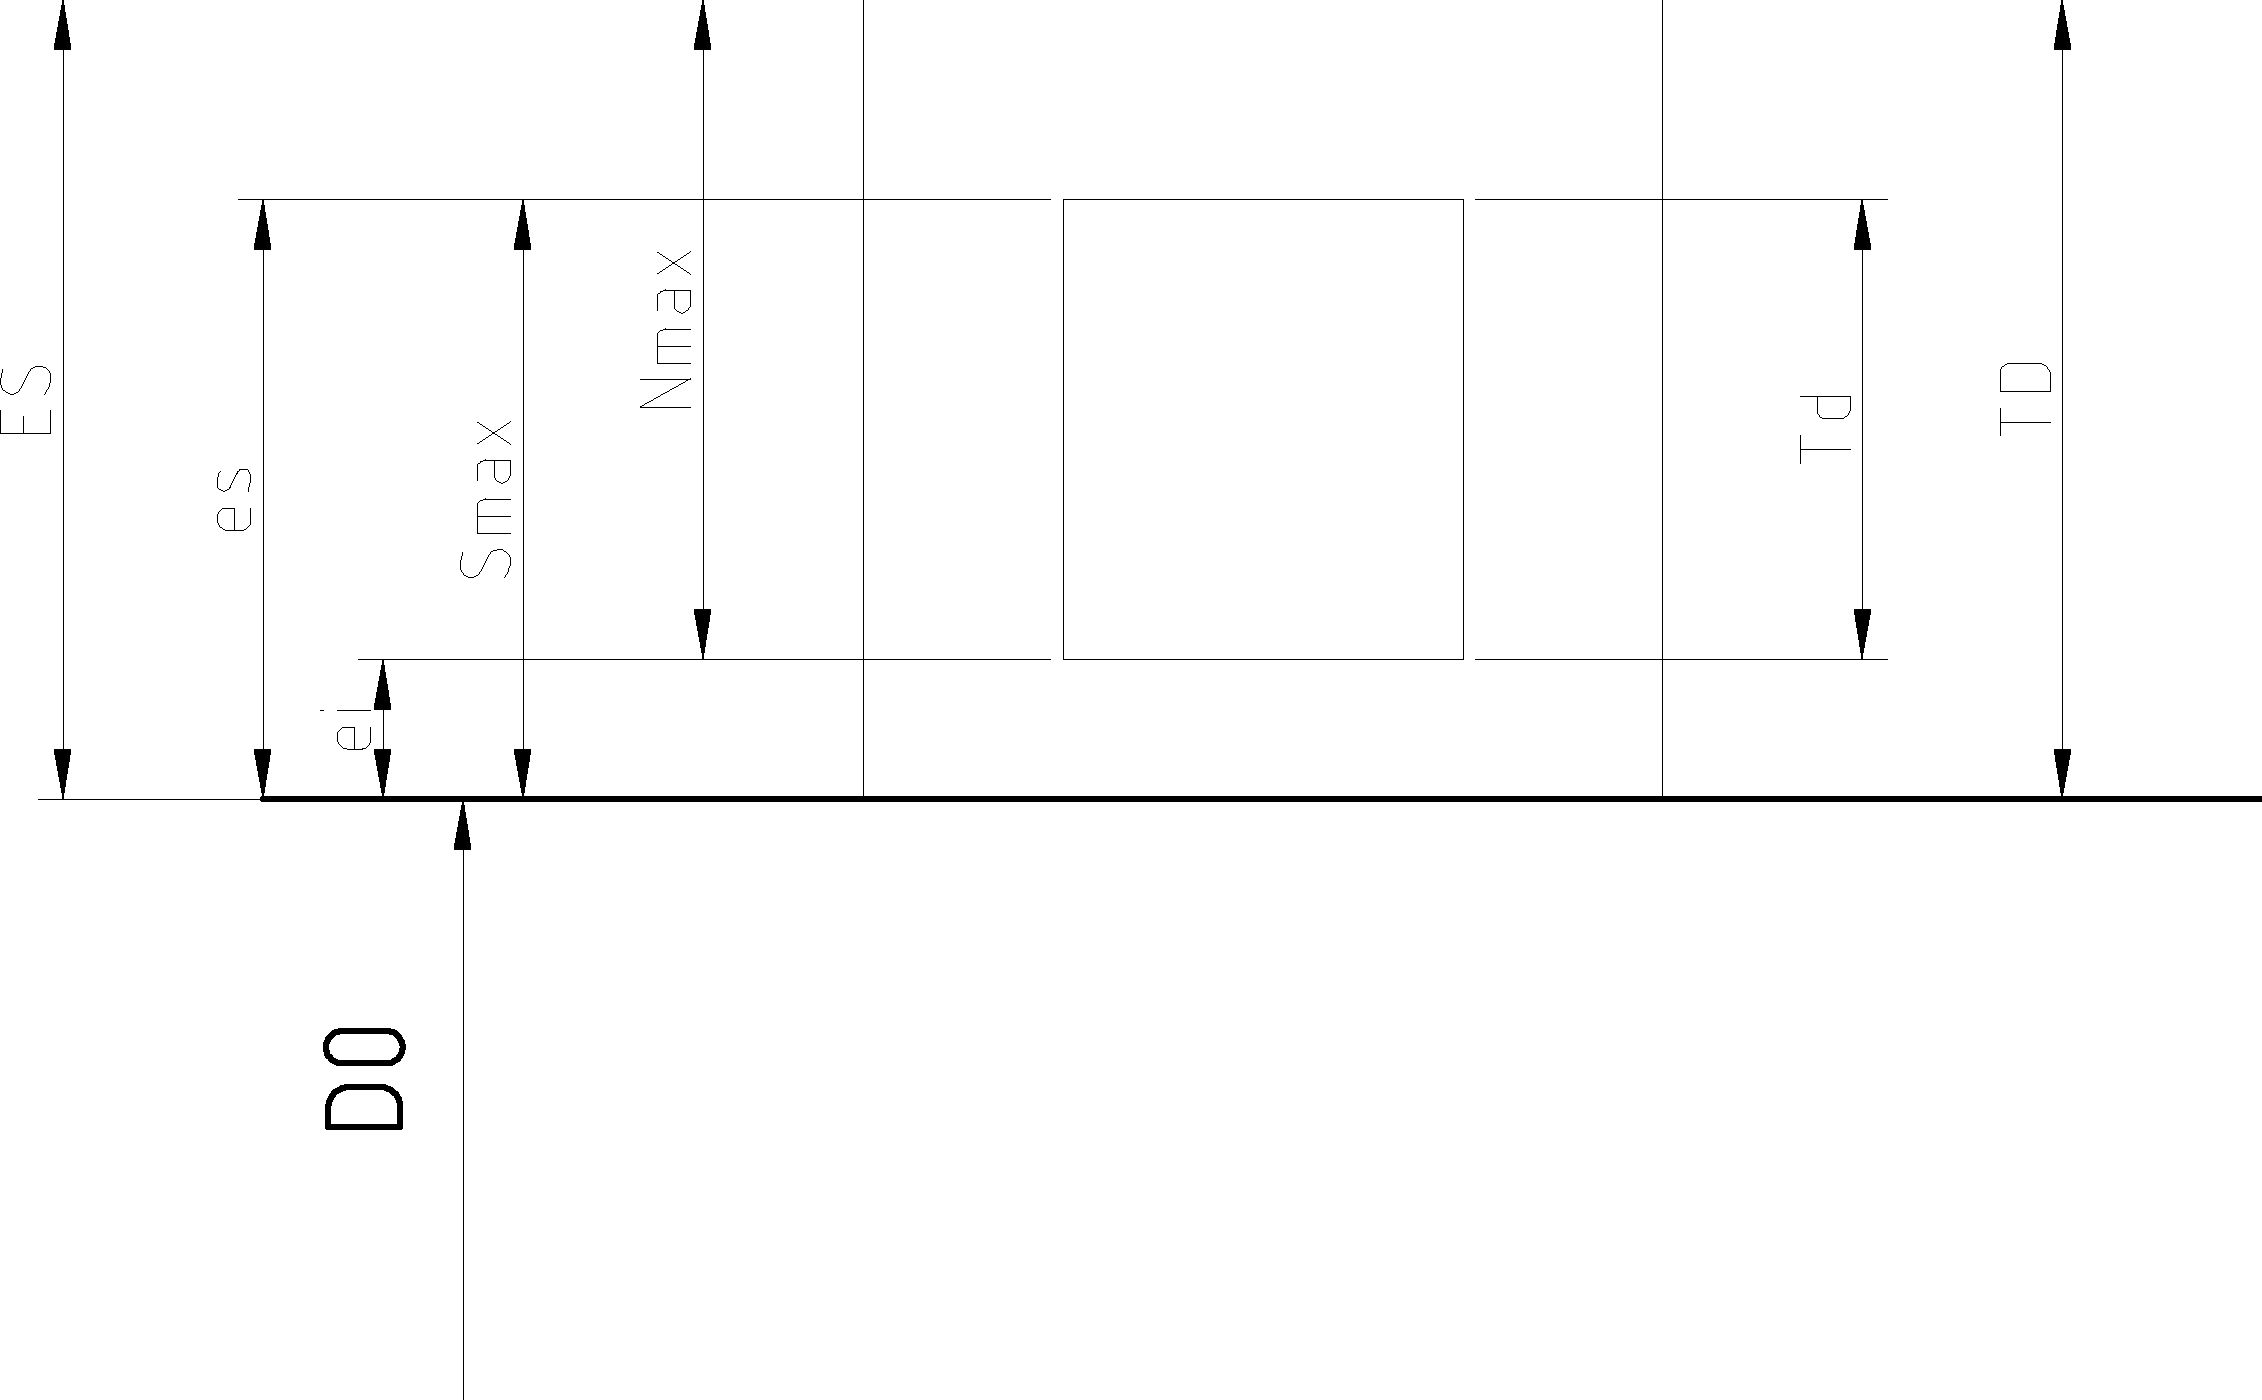
\includegraphics[width=0.7\linewidth]{pic/1_1}
	\caption{Посадка с натягом}
	\label{fig:11}
\end{figure}


\section{Характеристики системы допусков и посадок главных цилиндрических соединений}

\begin{enumerate}
	\item Обеспечение нормального температурного режима: $t_{дет} = t_{изм}$ --- совместная выдержка детали и измерительного средства
	\item Единица допуска --- связывает точность с самим размером (устанавливают экспериментально). $IT = k \cdot i$, $i = 0.45 \sqrt[3]{D} + 0.001D$
	\item Квалитет --- совокупность допусков, характеризуемых постоянной относительной точностью, определяемый коэффициентом $k$, для всех номинальных размеров данного диапазона.
	\item Ряд допусков --- строится на основании единицы допуска и квалитета точности.
	\item Диаметры по интервалам распределены так, чтобы допуски, рассчитанные по крайним значениям диаметров и средним отличалось бы не более, чем на 5-8\%.
\end{enumerate}

\section{Основные отклонения валов и отверстий}

Основным отклонением называется одно из двух предельных, ближе расположенное к нулевой линии.

\begin{figure}
	\centering
	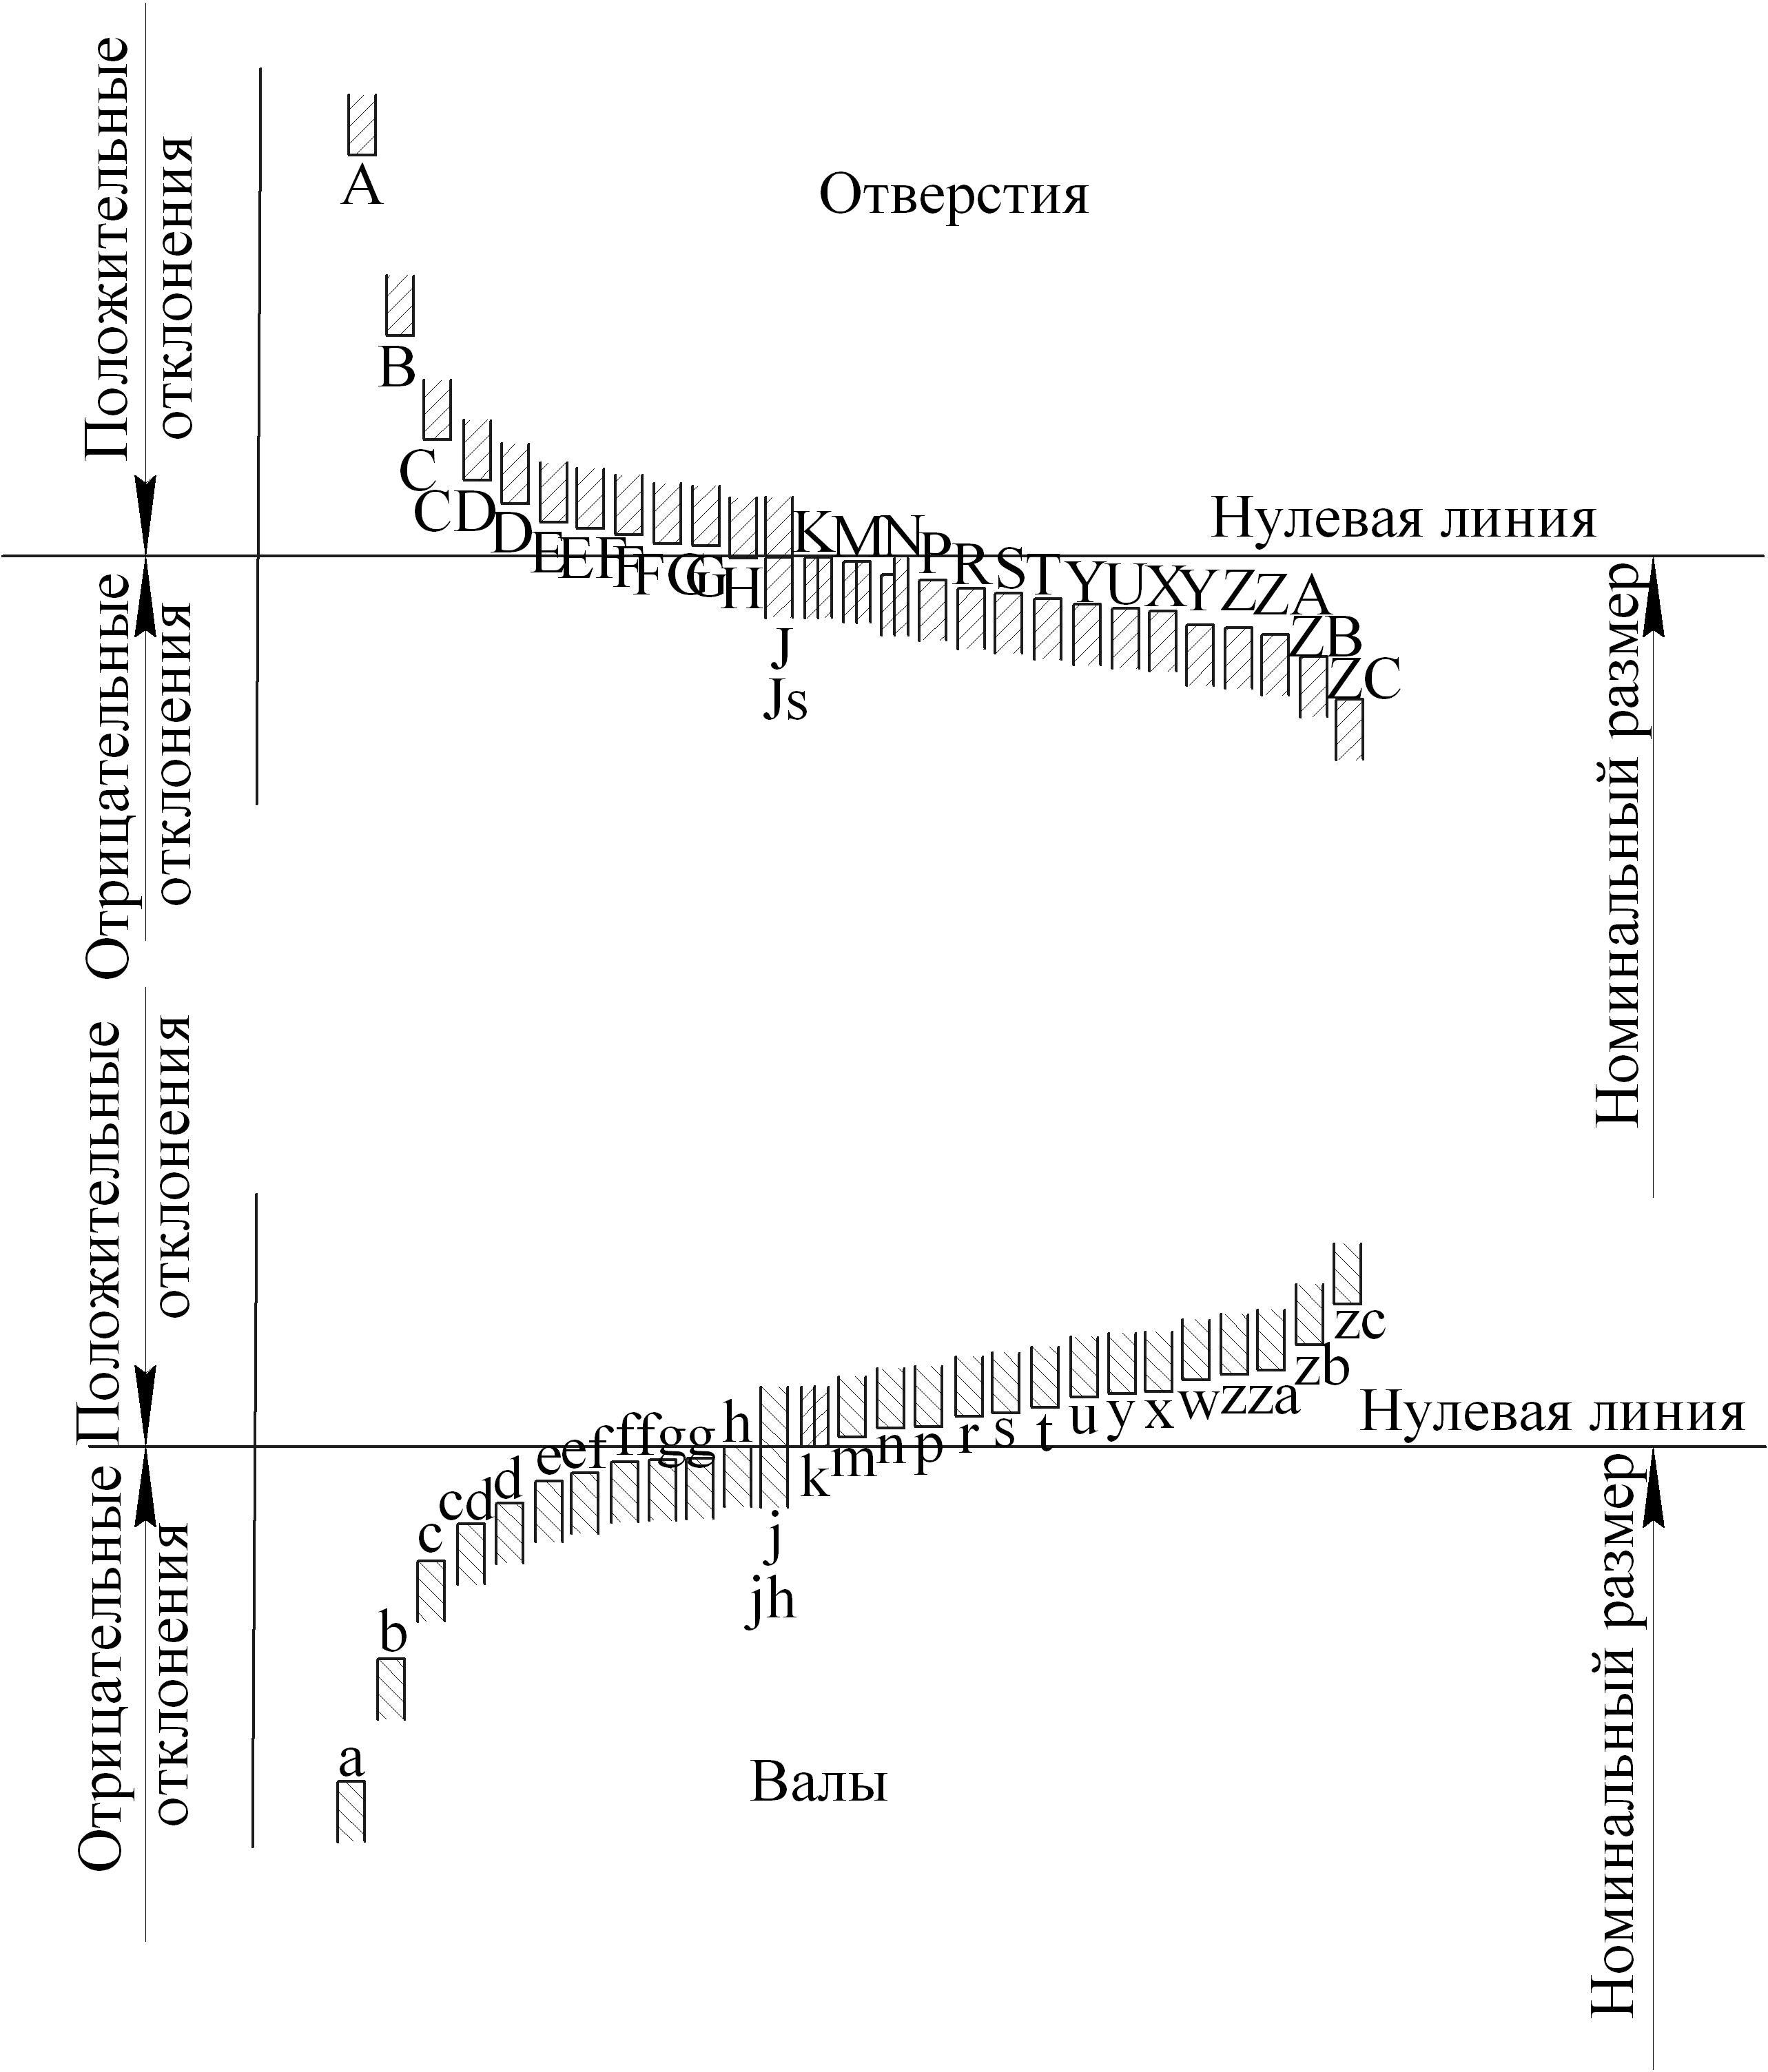
\includegraphics[width=0.7\linewidth]{pic/1_3}
	\caption{Основные отклонения валов и отверстий}
	\label{fig:13}
\end{figure}

 Основные отклонения отверстий построены таким образом, чтобы обеспечить образование посадок в системе вала, аналогичным посадкам в системе отверстия. Основные отклонения отверстий равны по величине и противоположны по знаку основным отклонениям валов, обозначаемым той же буквой. Основные отклонения отверстий определяются по двум правилам.

Общее правило. Основное отклонение отверстия должно быть симметрично относительно нулевой линии основному отклонению вала, обозначаемому той же буквой: EI = – es для A – H; ES = – ei – для J – ZC.

Специальное правило. Две соответствующие друг другу посадки в системе отверстия и в системе вала, в которых отверстие данного квалитета соединяется с валом ближайшего более точного квалитета, должны иметь одинаковые зазоры или натяги (например, H7/p6 и P7/h6).

\section{Три типа посадок}

\begin{enumerate}
	\item Посадка с зазором --- посадка, при которой в соединении, всегда образуется зазор, т.е. наименьший предельный размер отверстия больше наибольшего предельного размера вала или равен ему.
	
	Наименьший зазор ($S_{\min}$) – разность между наименьшим предельным размером отверстия и наибольшим предельным размером вала в посадке с зазором:
	
	$$S_{\min} = D_{\min} – d_{\max} = EI – es$$
	
	Наибольший зазор ($_{S\max}$) – разность между наибольшим предельным размером отверстия и наименьшим предельным размером вала в посадке с зазором или в переходной посадке
	
	$$S_{\max} = D_{\max} – d_{\min} = ES – ei$$
	
	Средний зазор ($S_c$) – это среднее арифметическое наибольшего и наименьшего зазоров.
	
	\item Посадка с натягом - посадка, при которой в соединении всегда образуется натяг, т.е. наибольший предельный размер отверстия меньше наименьшего предельного размера вала или равен ему.
	
	Наименьший натяг ($N_{\min}$) – разность между наименьшим предельным размером вала и наибольшим предельным размером отверстия до сборки в посадке с натягом:.
	
	$$N_{\min} = d_{\min} – D_{\max} = ei – ES$$
	
	Наибольший натяг ($N\max$) – разность между наибольшим предельным размером вала и наименьшим предельным размером отверстия до сборки в посадке с натягом или в переходной посадке:
	
	$$N_{\max} = d_{\max} – D_{\min} = es – EI$$
	
	Средний натяг ($N_c$) – это среднее арифметическое наибольшего и наименьшего натягов
	
	\item 	Переходная посадка - посадка, при которой в соединении возможно получение как зазора, так и натяга, в зависимости от действительных размеров отверстия и вала.
	
	Переходная посадка характеризуется наибольшими значениями натяга ($N_{\max}$) и зазора ($S_{\max}$)
\end{enumerate}

\begin{figure}
	\centering
	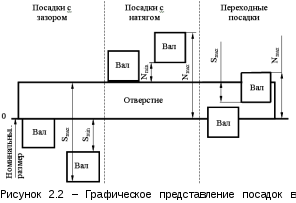
\includegraphics[width=0.7\linewidth]{pic/1_4}
	\caption{Три типа посадок}
	\label{fig:14}
\end{figure}

\section{Посадки в системе отверстия}

Посадки в системе отверстия – посадки, в которых требуемые зазоры и натяги получаются сочетанием различных полей допусков валов с полем допуска основного отверстия, обозначаемого буквой H. Основное отверстие – отверстие, нижнее отклонение которого равно нулю.

\section{Посадки в системе вала}

Посадки в системе вала – посадки, в которых требуемые зазоры и натяги получаются сочетанием различных полей допусков отверстий с полем допуска основного вала, обозначаемого буквой h. Основной вал – вал, верхнее отклонение которого равно нулю.

\section{Посадки с зазором}

Посадки с зазором предназначены для подвижных и неподвижных соединений. Посадки рассчитаны на следующие условия их применения: нормальный температурный режим работы, близкие коэффициенты линейных расширений материалов деталей.

\section{Посадки с натягом}

 Посадки применяются только в точных квалитетах, используются для передачи крутящих моментов и осевых сил без дополнительного крепления.

Посадки предназначены для неподвижных и неразъемных соединений. Относительная неподвижность обеспечивается силами трения, возникающими на контактирующих поверхностях вследствие упругой деформации, создаваемой натягом при сборке соединения.

\section{Переходные посадки}

 Переходные посадки применяются только в точных квалитетах – с 4-го по 8-й и используются как центрирующие посадки. Предназначены для неподвижных, но разъемных соединений, так как обеспечивают легкую сборку и разборку соединения.

Переходные посадки требуют, как правило, дополнительного крепления соединяемых деталей.

\section{Посадки подшипников качения}

В зависимости от условий работы узла или механизма в целом различают местное, циркуляционное и колебательное нагружения колец подшипников. При местном нагружении кольцо неподвижно и нагрузка направлена и действует на одно и то же место в кольце. При циркуля­ционном нагружении за каждый оборот подшипника последовательно нагружаются все участки окружности дорожки качения кольца. При колебательном нагружении лишь определенный участок кольца пооче­редно подвергается нагрузке.

Соединение вращающихся относительно нагрузки колец с валом или корпусом выполняют обязательно с натягом.

Предельные отклонения размеров посадочных поверхностей подшип­ников класса точности 0 регламентированы ГОСТ 520-89 «Подшипники качения. Технические требования». Посадки подшипников отличаются от обычных расположением и величинами полей допусков на поса­дочные поверхности колец.

\section{Отклонение формы поверхностей}

Реальная поверхность --- поверхность, ограничивающая деталь и полученная в результате обработки.

Номинальная поверхность --- идеальная поверхность, номинальная форма которой задана на чертеже.

Действительная поверхность --- поверхность, воспроизведенная по размерам, измеренным с допусками.

Прилегающая поверхность: имеет форму номинальной поверхности; соприкасается с реальной поверхностью; расположена вне материала так, что расстояние до наиболее удаленной точки реальной поверхности минимально (расстояние измеряется по нормали и прилегающей поверхности).

\begin{tabular}{|c|c|}
	\hline 
	Вид допуска формы & Обозначение \\ 
	\hline 
	Допуск прямолинейности & 
\includegraphics{pic/dop_form/index.jpg}  \\ 
	\hline 
	Допуск плоскостности & 
\includegraphics{pic/dop_form/get.jpg}  \\ 
	\hline 
	Допуск круглости & 
\includegraphics{pic/dop_form/index1.jpg} \\ 
	\hline 
	Допуск цилиндричности & 
\includegraphics{pic/dop_form/index2.jpg} \\ 
	\hline 
	Допуск профиля продольного сечения & 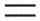
\includegraphics{pic/dop_form/get1.jpg} \\ 
	\hline 
\end{tabular} 

Отклонение от прямолинейности --- область на плоскости, ограниченная двумя параллельными прямыми, расположенными друг от друга на расстоянии, равном допуску прямолинейности Т.

Отклонение плоскостности --- наибольшее расстояние от точек реальной поверхности (профиля) до прилегающей плоскости (прямой) в пределах нормируемого участка

Отклонение от круглости --- наибольшее расстояние от точек реального профиля до прилегающей окружности.

Прилегающая окружность --- окружность минимального диаметра, описанная вокруг реального профиля наружной поверхности вращения, или окружность максимального диаметра, вписанная в реальный профиль внутренней поверхности. 

Отклонение от цилиндричности - наибольшее расстояние от точек реальной поверхности до прилегающего цилиндра в приделах нормируемого участка.

Отклонение от профиля продольного сечения - наибольшее расстояние от точек образованной реальной поверхности и лежащих в плоскости проходящей через ось до соответствующей стороны прилегающего профиля. В приделах нормируемого участка.

\section{Отклонения расположения поверхностей и осей}

\begin{tabular}{|c|c|}
	\hline 
	Допуски расположения & Обозначение \\ 
	\hline 
	Допуск параллельности & 
\includegraphics{pic/dop_rasp/index.jpg}  \\ 
	\hline 
	Допуск перпендикулярности & 
\includegraphics{pic/dop_rasp/index1.jpg} \\ 
	\hline 
	Допуск наклона & 
\includegraphics{pic/dop_rasp/index2.jpg} \\ 
	\hline 
	Допуск соосности & 
\includegraphics{pic/dop_rasp/index4.jpg} \\ 
	\hline 
	Допуск симметричности & 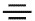
\includegraphics{pic/dop_rasp/index6.jpg} \\ 
	\hline 
	Позиционный допуск & 
\includegraphics{pic/dop_rasp/index7.jpg} \\ 
	\hline 
	Допуск пересечения осей & 
\includegraphics{pic/dop_rasp/index8.jpg} \\ 
	\hline 
\end{tabular} 

Отклонение от параллельности(EPA) --- разность наибольшего и наименьшего расстояний между плоскостями в пределах нормируемого участка.

Отклонение от перпендикулярности плоскостей(EPR) --- отклонение угла между плоскостями от прямого угла, выраженное в линейных единицах на длине нормируемого участка.

Отклонение наклона (EPN):отклонение угла между рассматриваемым элементом (плоскостью, осью) и базой от номинального угла, выраженное в линейных единицах на длине нормируемого участка.

Отклонение от соосности (EPC):наибольшее расстояние между осью рассматриваемой поверхности вращения и базой (осью базовой поверхности или общей осью двух или нескольких поверхностей) на длине нормируемого участка.

Отклонение от симметричности (EPS):наибольшее расстояние между плоскостью симметрии (осью) рассматриваемого элемента (элементов) и базой – плоскостью симметрии базового элемента, осью или общей плоскостью симметрии двух или нескольких элементов в пределах нормируемого участка.

Позиционное отклонение (EPP):наибольшее расстояние между реальным расположением элемента (его центра, оси или плоскости симметрии) и его номинальным расположением в пределах нормируемого участка.

Отклонение от пересечения осей (EPX):наименьшее расстояние между осями, номинально пересекающимися.


	
	\section{Шероховатость}

Шероховатость поверхности --- совокупность неровностей поверхности с относительно мальми шагами, выделенную с помощью базовой длины. Появляется в процессе формообразования.

$R_a$ --- среднее арифметическое отклонение профиля.

\[ R_a = \dfrac{1}{l} \int\limits_0^l |y(x)| \; dx \]

$R_z$ --- высота неровностей профиля по 10 точкам. 5 --- наибольшие выступы, 5 --- наибольшие впадины.

\[ R_z = \dfrac{\sum\limits_{i=1}^5 |y_{pi}| - \sum\limits_{i=1}^5 |y_{vi}|}{5} \]

$R_{\max}$ --- наибольшая высота неровностей профиля. Расстояние между линией выступов профиля и линией впадин профиля.

$S_m$ --- средний шаг неровностей профиля --- среднее значение неровностей профиля в пределах базовой длины.

\begin{figure}
	\centering
	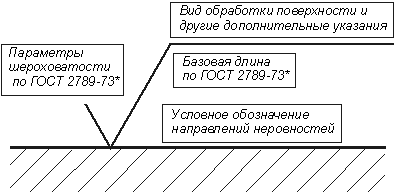
\includegraphics[width=0.7\linewidth]{pic/1_5}
	\caption{Обозначение шероховатости}
	\label{fig:15}
\end{figure}


$S$ --- Средний шаг выступов профиля --- среднее значение выступов профиля в пределах базовой длины.

$t_p$ --- Относительная опорная длина профиля --- отношение опорной длины профиля к базовой длине.

\[ t_p = \dfrac{1}{l} \sum\limits_{i=1}^n b_i \]

\begin{figure}
	\centering
	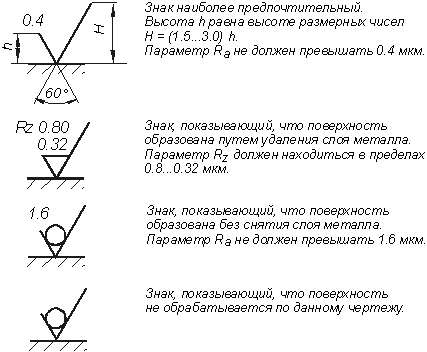
\includegraphics[width=0.7\linewidth]{pic/1_6}
	\caption{Обозначение шероховатости на чертеже.}
	\label{fig:16}
\end{figure}


\section{Резьбовые соединения.}

Приведенный средний диаметр резьбы --- средний диаметр воображаемой идеальной резьбы, которая имеет те же шаг и угол наклона боковых сторон, что и основной или номинальный профиль резьбы, и длину, равную заданной длине свинчивания, которая плотно (без взаимного смещения или натяга) соприкасается с реальной резьбой по боковым сторонам резьбы. Необходим для упрощения допусков контроля резьбы.

\[ d_{2 пр} = d_{2 изм} + f_p + f_{\alpha} \]

\[  D_{2 пр} = D_{2 изм} - (f_p + f_{\alpha})  \]

$f_p$ --- диаметральная компенсация погрешности шага.

Средний диаметр, шаг и угол профиля являются основными параметрами резьбы, т.к. они определяют характер контакта резьбового соединения. Однако вследствие взаимосвязи между отклонениями шага, угла профиля и собственно среднего диаметра допустимые отклонения этих параметров раздельно не нормируют. Устанавливают только суммарный допуск на средний диаметр болта $Td_2$ и гайки $TD_2$, который включает допустимое отклонение собственно среднего диаметра $\bigtriangleup d_2$ и диаметральные компенсации погрешности шага и угла профиля, т.е.

\[ TD_2 = \bigtriangleup D_2 + f_p + f_{\alpha} \]

Условия годности резьбы:

\[ d_{2 изм} \geqslant d_{2 \min}; d_{2 пр} \leqslant d_{2 \max} \]

Пример обозначения резьбы: М12-6g(наружняя); M12-6H(внутренняя)

\section{Зубчатые передачи}

Классификация зубчатых передач:

\begin{enumerate}
	\item Отсчётные --- зубчатые передачи различных счётных механизмов. Основное требование --- высокая кинематическая точность.
	\item Скоростные --- требуется плавность работы.
	\item Силовые --- зубчатые передачи в прокатных станах. Требуется полнота контакта сопряжённых зубьев
\end{enumerate}

Установлено 12 степеней точности.

Нормы точности:

\begin{enumerate}
	\item Кинематическая --- устанавливает разность между действительными и номинальными углами поворота колеса
	\item Плавность работы --- ограничивает погрешность угла поворота колеса при повороте на 1 зуб.
	\item Контактная точность --- Ограничивают неполноту контакта сопряжённых зубьев
\end{enumerate}

Погрешность передаточного отношения:

\[ F_{ior} = (\varphi_{2 действ} - \varphi_{2 ном}) \cdot r [мкм] \]

\begin{figure}
	\centering
	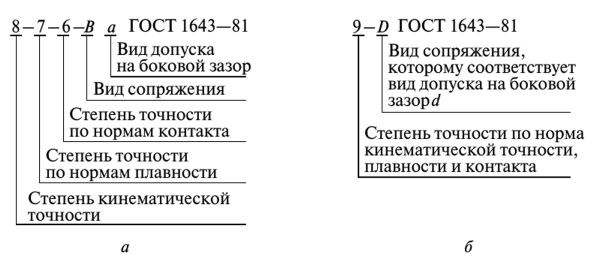
\includegraphics[width=0.7\linewidth]{pic/408}
	\caption{Обозначение точности зубчатого колеса}
	\label{fig:408}
\end{figure}

Принцип комбинирования норм точности --- для одного колеса можно назначать разные точности на разные параметры. Упрощает производство, т. к. последняя операция может улучшать только 1 показатель.

Виды сопряжений зубьев зубчатых колес в передачах

Характер сопряжений зубьев определяется боковым зазором между их нерабочими боковыми поверхностями.

Боковой зазор в передаче отсчитывают по общей нормали к боковым поверхностям зубьев (по линии зацепления). Он необходим для компенсации погрешностей изготовления и сборки передач, для создания расчетных условий смазывания, а также для устранения опасности заклинивания зубьев одного зубчатого колеса во впадинах другого в результате тепловых и силовых деформаций.


	
	\section{Измерения}

Прямое измерение – это измерение, измерение в котором искомое значение величины находят непосредственно из опытных данных.

Косвенное измерение – искомую величину находят по известной зависимости между искомой величиной и величинами, определяемыми прямыми измерениями.

Методы измерения:

Метод непосредственной оценки – значение величины определяется непосредственно по отсчетному устройству измерительного прибора.
Для этого необходимо, чтобы диапазон показаний шкалы был больше значения измеряемой величины.
\[  ДП>L  \]
При методе непосредственной оценки (НО) настройку прибора на нуль производят по базовой поверхности прибора. Под действием различных факторов (изменения температуры, влажности, вибраций и т.д.) может произойти смешение нуля. Поэтому периодически необходимо производить проверку и соответствующую регулировку.

Метод сравнения – измеряемую величину сравнивают с величиной, воспроизводимой мерой. При измерении методом сравнения с мерой результатом наблюдения является отклонение измеряемой величины от значения меры. Значение измеряемой величины получают алгебраическим суммированием значения меры и отклонения от этой меры, определенного по показанию прибора.

\[ L = M + П \]

Случайные погрешности измерения --- погрешность, изменяющая величину и знак в зависимости от случайных обстоятельств.

Случайные погрешности подчиняются закону распределения Гаусса:

\[ P(x) = \dfrac{1}{G \sqrt{2 \pi}} e^{-\frac{(x - \mu)^2}{2 G^2}} \]

Систематическая погрешность --- погрешность, постоянная по определённому закону при повторных применениях.

 Результаты наблюдений, полученные при наличии систематической погрешности, называются неисправленными. При проведении измерений стараются в максимальной степени исключить или учесть влияние систематических погрешностей. Это может быть достигнуто следующими путями:

\begin{itemize}
	\item устранением источников погрешностей до начала измерений. В большинстве областей измерений известны главные источники систематических погрешностей и разработаны методы, исключающие их возникновение или устраняющие их влияние на результат измерения. В связи с этим в практике измерений стараются устранить систематические погрешности не путем обработки экспериментальных данных, а применением СИ, реализующих соответствующие методы измерений;
	
	\item определением поправок и внесением их в результат измерения;
	
	\item оценкой границ неисключенных систематических погрешностей.
\end{itemize}

\section{Контроль}

Калибры – средства измерительного контроля, предназначенные для проверки соответствия действительных размеров, формы и расположения поверхностей деталей заданным требованиям.

Калибры применяют для контроля деталей в массовом и серийном производствах. Калибры бывают нормальные и предельные.

Нормальный калибр – однозначная мера, которая воспроизводит среднее значение (значение середины поля допуска) контролируемого размера. При использовании нормального калибра о годности детали судят, например, по зазорам между поверхностями детали и калибра, либо по «плотности» возникающего сопряжения между контролируемой деталью и нормальным калибром. Оценка зазора, следовательно, результаты контроля в значительной мере зависят от квалификации контролера и имеют субъективный характер.

Предельные калибры – мера или комплект мер обеспечивающие контроль геометрических параметров деталей по наибольшему и наименьшему предельным значениям. Изготавливают предельные калибры для проверки размеров гладких цилиндрических и конических поверхностей, глубины и высоты уступов, параметров резьбовых и шлицевых поверхностей деталей. Изготавливают также калибры для контроля расположения поверхностей деталей, нормированных позиционными допусками, допусками соосности и др.

При контроле предельными калибрами деталь считается годной, если проходной калибр под действием силы тяжести проходит, а непроходной калибр не проходит через контролируемый элемент детали. Результаты контроля практически не зависят от квалификации оператора.

По конструкции калибры делятся на пробки и скобы. Для контроля отверстий используют калибры-пробки, для контроля валов – калибры-скобы.

Обозначение на чертеже: $ ПР=60,0065_{-0.0012} $

\section{Техническое регулирование}

 Техническое регулирование – правовое регулирование отношений при установлении, применении и исполнении обязательных требований к объектам технического регулирования, добровольных требований к объектам технического регулирования, выполнению работ или оказанию услуг и правовому регулированию отношений при оценке соответствия.

Документ, осуществляющий это регулирование – технический регламент, документ, имеющий силу закона РФ, который и устанавливает обязательные для применения требования к объектам технич. регулирования.

Объекты технического регулирования:
\begin{itemize}
	\item продукция, в т.ч. здания, строения и сооружения;
	
	\item процессы проектирования (в т.ч. изыскания), производства, строительства, монтажа, наладки, эксплуатации, хранения, перевозки, реализации и утилизации.
\end{itemize}

 Техническое регулирование направлено на отношения, возникающие:

\begin{enumerate}
	\item  при разработке, принятии, применении и исполнении обязательных требований к объектам технического регулирования;
	
	\item  разработке, принятии, применении и исполнении на добровольной основе требований к объектам технического регулирования, выполнению работ или оказанию услуг;
	
	\item  оценке соответствия.
\end{enumerate}

Контроль (надзор) за соблюдением требований ТР – проверка выполнения юридическим лицом или индивидуальным предпринимателем требований ТР к продукции или связанным с ними процессам ЖЦП и принятие мер по результатам проверки.

\section{Стандартизация}

Принцип предпочтительности --- один из основных принципов, используемых в стандартизации. Различают качественный и количественный аспекты применения этого принципа. Качественный аспект состоит в образовании предпочтительных рядов объектов стандартизации. Предпочтительность устанавливают для сложных объектов (изделий, деталей, процессов, типовых решений, обозначений), а также для их элементов (отдельных требований, параметров, норм точности и т.д.). Количественный аспект связан с построением числовых параметрических рядов.


	
\end{document}